\documentclass[aspectratio=169]{beamer}
\usepackage[utf8]{inputenc}

% packages
\usepackage{tikz}
\usepackage[spanish, es-nodecimaldot, es-tabla]{babel}
\usepackage{graphicx}
\usepackage{subfig}
\usepackage{bookmark}
% \usepackage{toc}
\usepackage{multimedia}
\usepackage{hyperref}
\usepackage{colortbl}
\usepackage{multicol}

% notes
\usepackage{pgfpages}
\setbeameroption{show notes on second screen=right}

\usetheme{Madrid}
\usecolortheme{beaver}

% Definir background
\setbeamertemplate{background}{
  \begin{tikzpicture}
    \useasboundingbox (0,0) rectangle(\the\paperwidth,\the\paperheight);
    \node[inner sep=0pt] at (0.5\paperwidth,0.1\paperheight) {
\includegraphics[width=\paperwidth,height=2cm]{template/banner_cimat.png}};
  \end{tikzpicture}
}

\title[Taller RL]{Taller de Aprendizaje por Refuerzo}
\author{Julio De La Torre Vanegas}
\institute[CIMAT]{Centro de Investigación en Matemáticas}

\date[2024]{\footnotesize \today}
\logo{
\includegraphics[height=1.5cm]{template/logo.png}}

\begin{document}
    \frame{\titlepage}

    \begin{frame}{Tabla de contenidos}
        % \begin{multicols}{3}
            \tableofcontents
        % \end{multicols}
    \end{frame}

    \section{Introducción}

        \begin{frame}{Aprendizaje por refuerzo}
            El aprendizaje por refuerzo tiene sus raíces en las teorías del condicionamiento y la psicología conductista, que estudian cómo los animales aprenden a partir de las consecuencias de sus acciones (30's).

            \begin{figure}
                \centering
                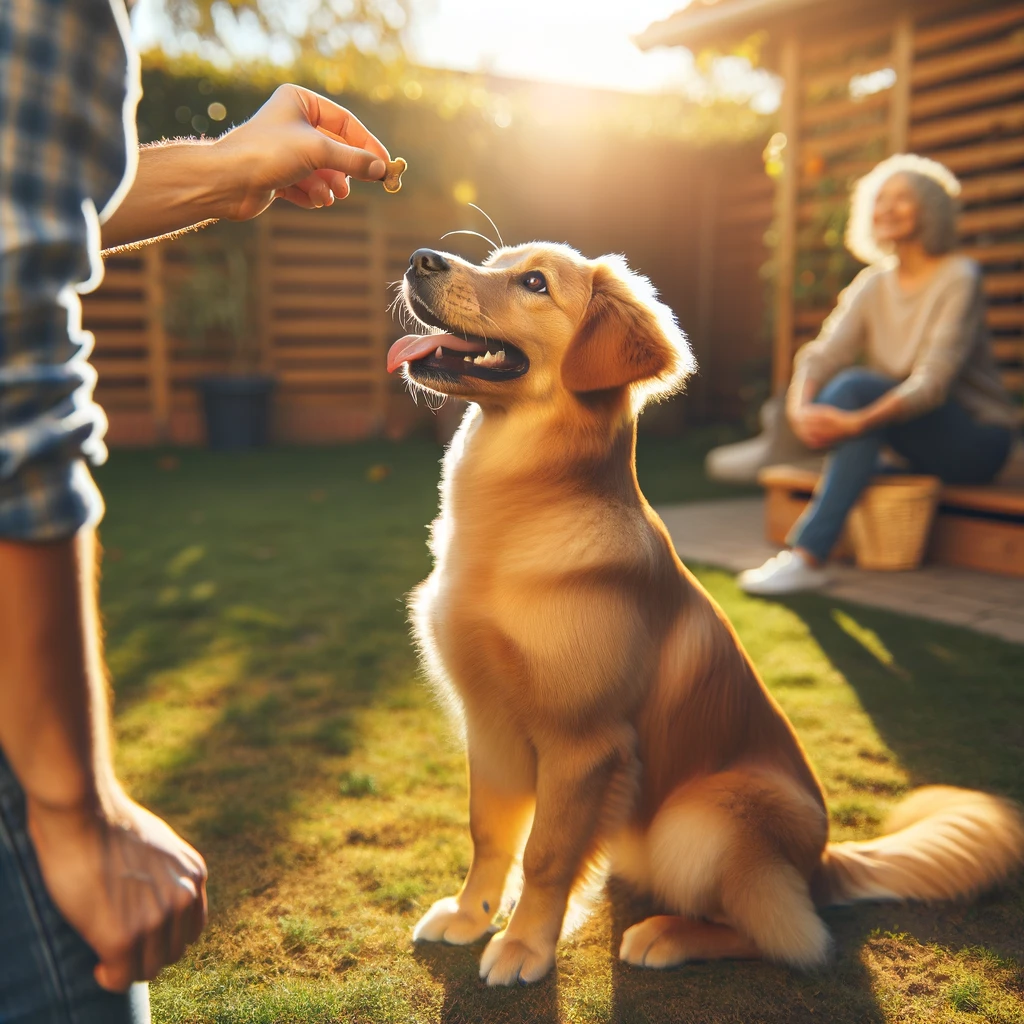
\includegraphics[height=0.5\textheight]{imgs/animal.png}
                \caption{Recompensa a la acción de sentarse}
            \end{figure}
        \end{frame}

        \begin{frame}{Aprendizaje por refuerzo}
           \begin{figure}
                \centering
                \subfloat[]{\movie[]{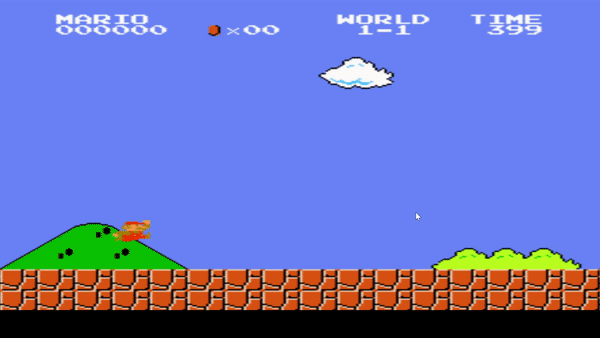
\includegraphics[height=0.3\textheight]{gifs/prev/mario_1.png}}{gifs/out/mario_1.gif}}
                \hspace{1cm}
                \subfloat[]{\movie[]{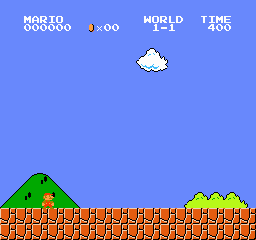
\includegraphics[height=0.3\textheight]{gifs/prev/mario_2.png}}{gifs/out/mario_2.gif}}
                \caption{Aprendizaje por refuerzo aplicado a videojuegos}
            \end{figure}
        \end{frame}

        \begin{frame}{Aprendizaje por refuerzo}
            \begin{figure}
                \centering
                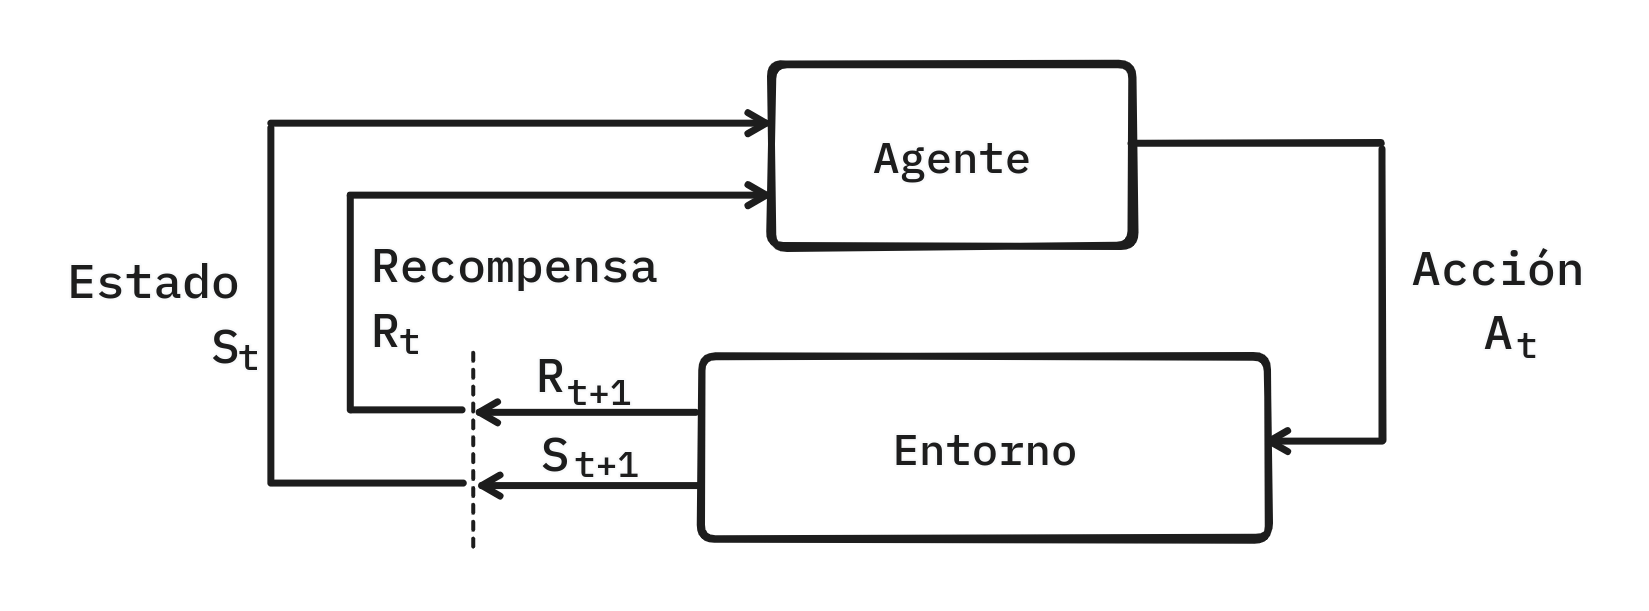
\includegraphics[height=0.5\textheight]{imgs/RL.png}
                \caption{Esquema del aprendizaje por refuerzo}
            \end{figure}
        \end{frame}
\end{document}